% BANKS-SOURCE: pdf=192 print=182 kind=figure id=9.9
% The seven one-loop Wilson-loop topologies (a)--(g) of the source figure.
% Every propagator is a native TikZ coil decoration so the figure stays
% editable.
\tikzset{
  BanksNWall/.style={line width=.55pt},
  BanksNGluon/.style={line width=.48pt,decorate,
    decoration={coil,aspect=.7,amplitude=4.6pt,segment length=#1}},
  BanksNGluon/.default=10pt,
  BanksNVertex/.style={fill=black,draw=black},
}

% The two static-source (Wilson-loop) lines bounding a panel.
\newcommand{\BanksNPanel}[2]{%
  \begin{scope}[shift={(#1,#2)}]
    \draw[BanksNWall] (-.95,-1.18)--(-.95,1.18);
    \draw[BanksNWall] (.95,-1.18)--(.95,1.18);
  \end{scope}%
}

% A gluon exchanged horizontally between the two static sources.
\newcommand{\BanksNHorizontal}[2]{%
  \draw[BanksNGluon] (#1-.95,#2)--(#1+.95,#2);
}

% Same, but traversed right-to-left so the lobes sit on the other side.
\newcommand{\BanksNHorizontalUp}[2]{%
  \draw[BanksNGluon] (#1+.95,#2)--(#1-.95,#2);
}

% Gluon emitted and reabsorbed by the left-hand static source.
\newcommand{\BanksNArchLeft}[2]{%
  \begin{scope}[shift={(#1,#2)}]
    \draw[BanksNGluon=9pt]
      (-.95,1.02) .. controls (.44,.96) and (.44,-.96) .. (-.95,-1.02);
  \end{scope}%
}

% The mirror graph, with the loop on the right-hand static source.
\newcommand{\BanksNArchRight}[2]{%
  \begin{scope}[shift={(#1,#2)}]
    \draw[BanksNGluon=9pt]
      (.95,-1.02) .. controls (-.44,-.96) and (-.44,.96) .. (.95,1.02);
  \end{scope}%
}

% Two crossed exchanged gluons.
\newcommand{\BanksNCross}[2]{%
  \begin{scope}[shift={(#1,#2)}]
    \draw[BanksNGluon=9.5pt] (-.95,.86)--(.95,-.86);
    \draw[BanksNGluon=9.5pt] (-.95,-.86)--(.95,.86);
  \end{scope}%
}

% The triple-gluon vertex graph.
\newcommand{\BanksNTriple}[2]{%
  \begin{scope}[shift={(#1,#2)}]
    \draw[BanksNGluon=9pt]
      (-.95,1.00) .. controls (-.44,1.06) and (-.10,.48) .. (.02,0);
    \draw[BanksNGluon=9pt]
      (-.95,-1.00) .. controls (-.44,-1.06) and (-.10,-.48) .. (.02,0);
    \draw[BanksNGluon=9pt] (.02,0)--(.95,0);
    \fill[BanksNVertex] (.02,0) circle (.055);
  \end{scope}%
}

% Exchanged gluon carrying a one-loop self-energy blob.
\newcommand{\BanksNInsertion}[2]{%
  \begin{scope}[shift={(#1,#2)}]
    \draw[BanksNGluon=10pt] (-.95,0)--(-.44,0);
    \draw[BanksNGluon=10pt] (.44,0)--(.95,0);
    \draw[fill=gray!45,line width=.48pt] (0,0) circle (.42);
  \end{scope}%
}

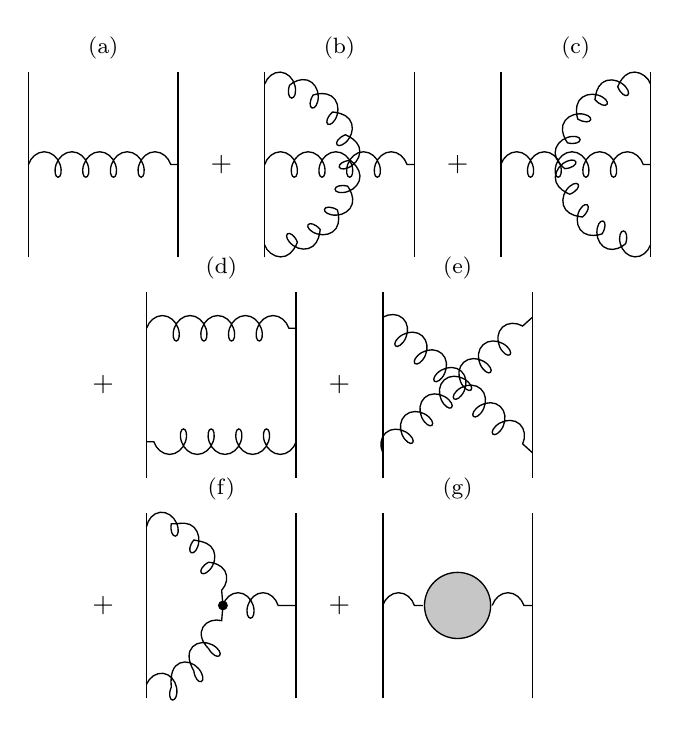
\begin{tikzpicture}[x=1cm,y=1cm,baseline=-.45ex]
  % Upper row: direct exchange and the two static-source self-energies.
  \BanksNPanel{0}{2.80}\BanksNPanel{3}{2.80}\BanksNPanel{6}{2.80}
  \BanksNHorizontal{0}{2.80}
  \BanksNHorizontal{3}{2.80}\BanksNArchLeft{3}{2.80}
  \BanksNHorizontal{6}{2.80}\BanksNArchRight{6}{2.80}

  % Middle row: the ladder and the crossed ladder.
  \BanksNPanel{1.5}{0}\BanksNPanel{4.5}{0}
  \BanksNHorizontal{1.5}{.72}\BanksNHorizontalUp{1.5}{-.72}
  \BanksNCross{4.5}{0}

  % Lower row: the triple-gluon vertex and the self-energy insertion.
  \BanksNPanel{1.5}{-2.80}\BanksNPanel{4.5}{-2.80}
  \BanksNTriple{1.5}{-2.80}\BanksNInsertion{4.5}{-2.80}

  \node at (0,4.28) {\footnotesize (a)};
  \node at (3,4.28) {\footnotesize (b)};
  \node at (6,4.28) {\footnotesize (c)};
  \node at (1.5,1.48) {\footnotesize (d)};
  \node at (4.5,1.48) {\footnotesize (e)};
  \node at (1.5,-1.32) {\footnotesize (f)};
  \node at (4.5,-1.32) {\footnotesize (g)};

  \node at (1.5,2.80) {$+$};
  \node at (4.5,2.80) {$+$};
  \node at (0,0) {$+$};
  \node at (3,0) {$+$};
  \node at (0,-2.80) {$+$};
  \node at (3,-2.80) {$+$};
\end{tikzpicture}
